%--------------------------------------------------
\section{Arquitectura de la aplicación}
La figura \ref{image:arquitectura} muestra la arquitectura general de la aplicación. En ella se pueden observar los diferentes módulos a desarrollar iniciando por las aplicaciones móviles para el cliente y el vendedor de las tiendas que se conectan a los Servicios REST del módulo de Gestión, Procesamiento y Proveedor de datos de Retail; de igual manera, de lado izquierdo se observa el panel de administración que hace uso de dichos servicios REST y estos a su vez realizan la conexión con el repositorio de datos de donde el módulo Generador de Registros Artificiales obtendrá la información.
\FloatBarrier
\begin{figure}[htbp!]
		\centering
			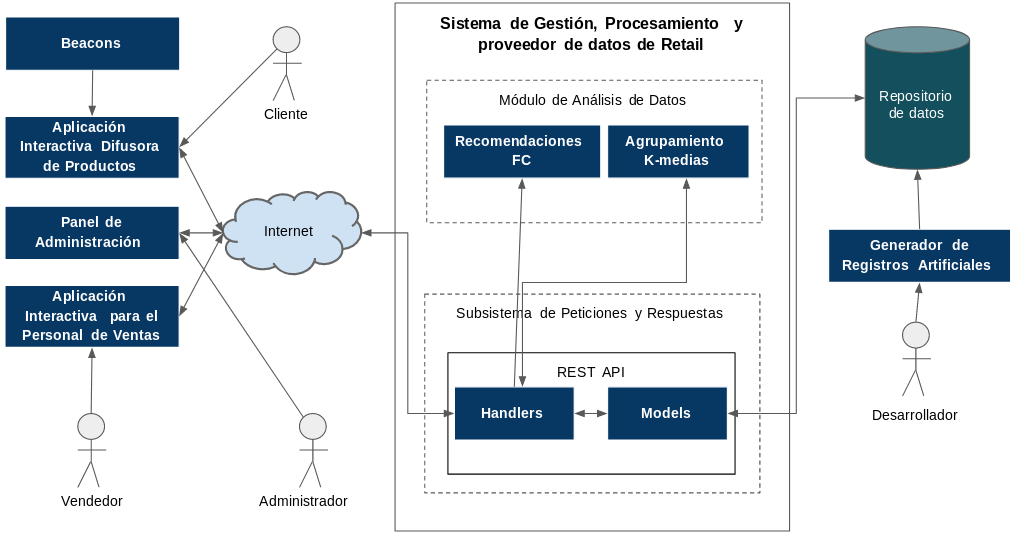
\includegraphics[width=.9 \textwidth]{imagenes/Arquitecturas/general}
		\caption{Arquitectura interna del sistema.}
		\label{image:arquitectura}
\end{figure}
\FloatBarrier

\begin{itemize}
\item \textbf{Panel de Administración.} Panel de administración enfocado para los usuarios administradores con el objetivo de proporcionar funcionalidades como: Alta de promociones y folletos, monitorear geográficamente Beacons y tiendas, actualizar información referente a éstos y ejecutar el algoritmo de K-medias para mejorar el clustering de clientes.  
\item \textbf{Aplicación Interactiva Difusora de Productos.} Prototipo de una aplicación móvil para los clientes en la cual se recibirán además de recomendaciones, anuncios, promociones y notificaciones.
\item \textbf{Aplicación Interactiva para el Personal de Ventas.} Prototipo de una aplicación móvil para los vendedores de la tienda con la que podrán dar una atención personalizada a los clientes ofreciendo recomendaciones de productos que sean de su interés o simplemente asesorarlos en su decisión de compra. 
\item \textbf{Módulo de Gestión, Procesamiento  y Proveedor de datos de Retail.}
\begin{itemize}
\item \textbf{Subsistema de peticiones y respuestas.}
\item \textbf{REST API.} 	Módulo encargado de manejar las peticiones y respuestas de las diferentes aplicaciones cliente.
\item \textbf{Módulo de análisis de datos.}

\begin{itemize}
\item \textbf{Algortitmo de agrupamiento K-medias.} Módulo que agrupa a los usuarios automáticamente dependiendo de sus características y gustos.
\item \textbf{Algoritmo de recomendaciones CF.} Módulo encargado de dar las recomendaciones basado en filtrado colavorativo sobre los usuarios al que cada usuario pertenece.
\end{itemize}

\item \textbf{Repositorio de datos.} Repositorio de datos PostgreSQL que almacena los datos del sistema.
\end{itemize}
\item \textbf{Generador de registros artificiales.} Módulo encargado de insertar registros ficticios en las diferentes entidades dentro del repositorio de datos del sistema.


\end{itemize}
